\chapter{Problem domain}
\chapterintro{This chapter details mechanisms and practises that ensures a requested Quality-of-Service level is met by a means of a self-adaptive system that scales across multiple service providers.}

\section{Self-adaptive system}

\subsection{Introduction}
What makes a concept of an adaptivity enticing is crucial idea behind guaranteeing Quality-of-Serivce: automatization. Generally, ensuring and enforcing given quality can be seen as continuous monitoring and reacting to events when necessary. Such idea can be expressed as IT process shown in figure \ref{fig:it-process}.

\begin{figure}[!ht]
  \begin{center}
    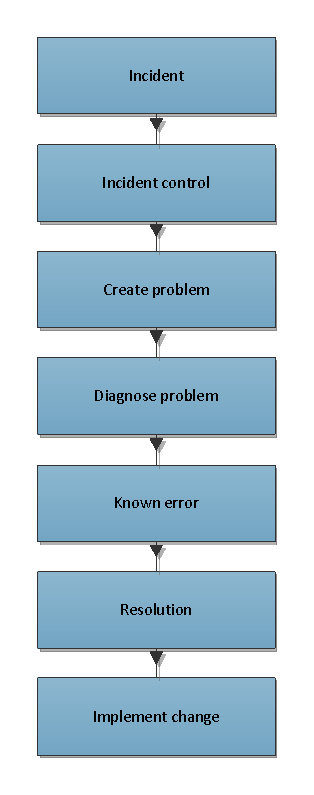
\includegraphics{chapter-adaptivity/it-process}
  \end{center}
  \caption{Exemplary IT process}
  \label{fig:it-process}
\end{figure}

While system administrator can be directly responsible for manually performing above-mentioned steps, it is much more favourable to automatize this process leading to a system self-management or an adaptable system. Not only does it lead to efficiency of an IT process but also to its effectiveness \cite{IBM06}. It is possible through:
\begin{itemize}
  \item \emph{rapid process initiation} - components auto-initiates actions based on information derived from a system
  \item \emph{reduced time and skill requirements} - automatization of IT processes makes them easier and less troublesome what is especially important for skill-intensive, error-prone and long lasting tasks
\end{itemize}

In a context of delivering a computing platform, adaptivity adds auto-scaling features to a solution offered by Platform-as-a-Service provider. Self-managing is possible through usage of an Elasticity Controller which gathers probes from resource such as application container and uses that knowledge to execute appropriate action on that resource, indirectly modifying consecutive probes \cite{VaRoBu11}. This concept illustrates diagram \ref{fig:elasticity-controller}.

\begin{figure}[!ht]
  \begin{center}
    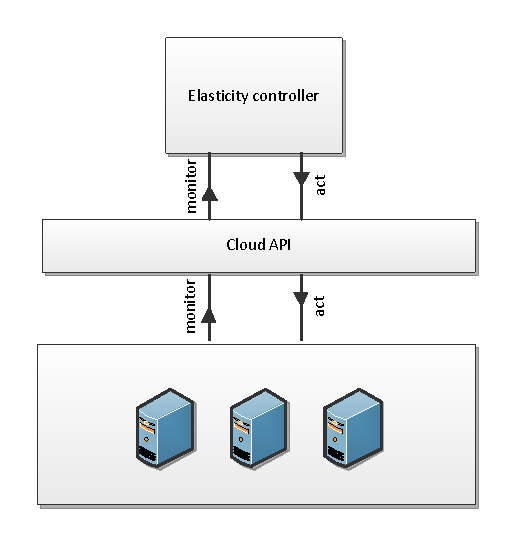
\includegraphics{chapter-adaptivity/elasticity-controller}
  \end{center}
  \caption{Elasticity controller}
  \label{fig:elasticity-controller}
\end{figure}

The remaining of this chapter describes crucial elements that compose elasticity controller: policies, data analysis, triggered actions and presents a comparison of cloud providers.
 
\subsection{Policies}
While auto-scaling is offered by a vast amount of cloud providers (e.g AWS, OpenShift, OpenNebula) it often lacks a sophisticated mechanisms allowing for specific scaling policies, being limited to only one predefined rule as it is in case of OpenShift for example. 
 
Policy denotes a condition which, when satisfied, triggers an action that is supposed to harness cloud instance in a way that future evaluations of condition will be unsuccessful. Typically condition itself is accompanied by a minimal and maximal number of node instances, allowing for ensuring minimal QoS and controlling maximal costs. Currently, industry leaders supports two main kind of policies \cite{AmazonAutoScaling}:
\begin{itemize}
 \item \textit{expression based} - allows to define how you to scale application in response to changing conditions, which include factors such as memory, CPU usage, cost or some indirect, calculated metrics
 \item \textit{scheduled} - allows to scale an application in response to predictable load changes. For example, traffic increases during the weekends and decreases on working days. Hence, that predictable traffic patterns is used to scale application based on current time.
\end{itemize}

Technically, policies are expressed in some human-readable format such as JSON, XML as it is in case of AWS EC2 or custom expression used for example by Carina. Appendix \ref{app:scaling-policies} presents example configuration used by AWS E2 Auto-Scaling.

\subsection{Data analysis}
Having policies defined, their conditions are evaluated against data acquired from sensors. In a simplest case this evaluation can be based on a Threshold Model \cite{LiWoZh05}, which defines a valid range. In cases when given metric violates that condition (i.e. value is either smaller than minimal or bigger than maximal acceptable) corresponding resource is properly adjusted - figure \ref{fig:threshold-model} illustrates that idea.

\begin{figure}[!ht]
  \begin{center}
    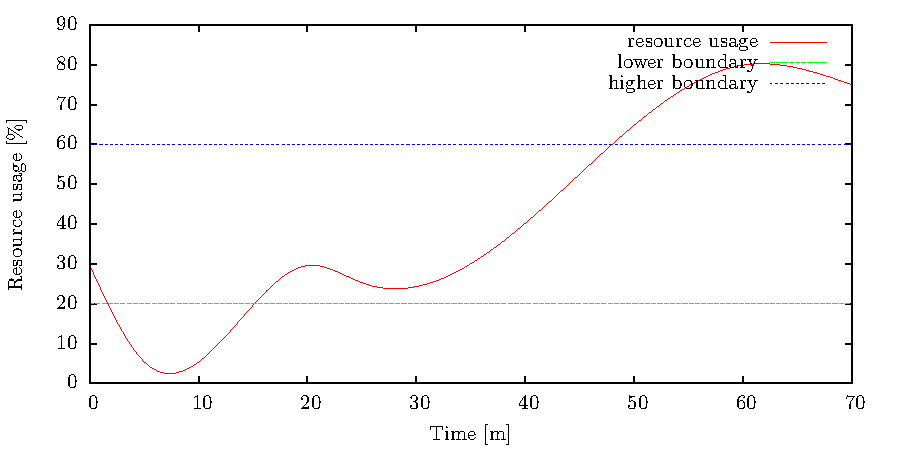
\includegraphics{chapter-adaptivity/threshold-model}
  \end{center}
  \caption{Threshold model}
  \label{fig:threshold-model}
\end{figure}

While trivial in its form, cases of AWS, OpenShift, Carina, OneCloud proves it is useful in a real-world scenarios. 

\subsection{Triggered actions}
Actions that are being triggered by a elasticity controller are focused on application scaling. Previous chapter described that problem in detail.



